\chapter{Реализация системы обработки данных} \label{chapt3}

Программная реализация алгоритмов мюонного скважинного плотномера выполнена с использованием программного пакета LabVIEW, библиотеки, написанной на языке C++ и алгоритмах, основанных на градиентном спуске, реализованных на матричном языке octave. 
На (\ref{img:operator}) представлен интерфейс оператора по вводу и обработке тарировочных данных. Тарировочные данные вводятся таблично. После введения данных проводится контроль их корректности.  При запуске начальной аппроксимации (кнопка «Аппроксимировать») отображается аппроксимационная кривая с наименьшей погрешностью, график погрешности в зависимости от текущего параметра и значение погрешности. При запуске оптимизационного алгоритма (кнопка <<Подстройка пар>>) отображается процент выполнения жадного алгоритма, график изменения погрешности, найденные компоненты аппроксимирующей суммы экспонент и числовое значение погрешности. Корректировка настроек алгоритма начальной аппроксимации и оптимизационного алгоритма производится через переключатели <<Изменить настройки>> и <<изменить коэффициенты>> соответственно. Переход на экран обработки измерений производится по кнопке <<Перейти на другой экран>>. Действия оператора по изменению данных и их сохранению контролируются. По выходу из программы (кнопка <<Конец работы>>) проверяется, есть ли несохраненные изменения, и в случае наличия таковых, оператору предлагается их сохранить.
 
\begin{figure} [h]
  \center
  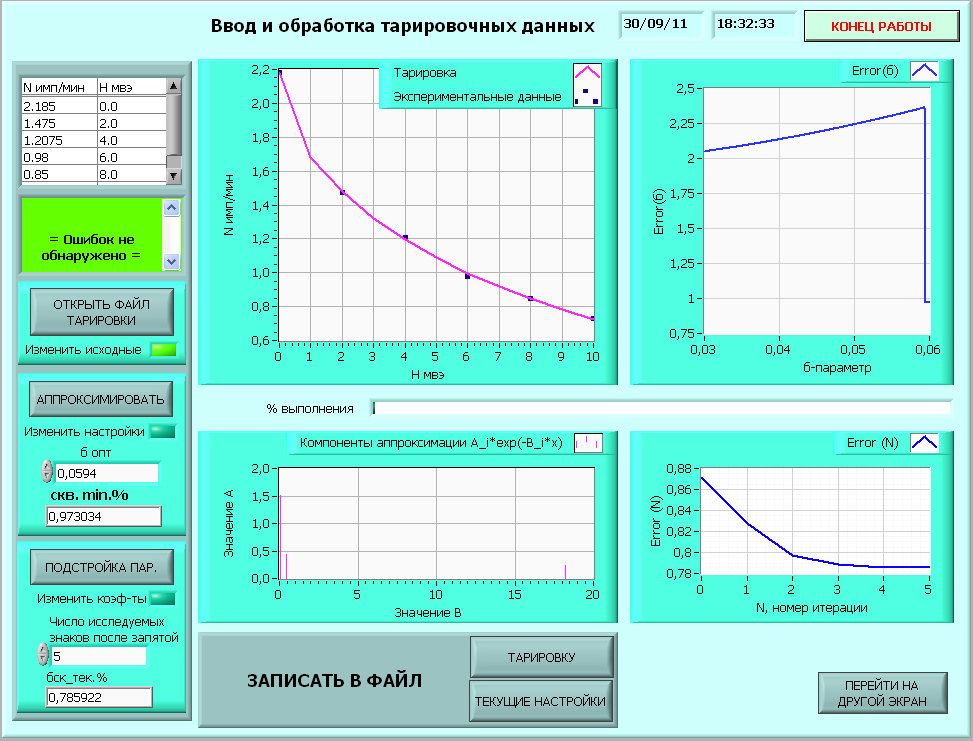
\includegraphics [scale=0.35] {operator}
  \caption{Интерфейс оператора по вводу и обработке тарировочных данных} 
  \label{img:operator} 

\end{figure}



Интерфейс оператора по обработке измерений (\ref{img:operator_results}) предоставляет возможность ввода измеренных данных, проверку их корректности, а также, графическое и табличное отображение результатов обработки. Введенные данные измерений и результат обработки  можно сохранить в файле, а также, вывести на принтер (кнопка <<Распечатать>>) или скопировать для экспорта в другое приложение (кнопка <<Копировать в буфер обмена>>).



\begin{figure} [h]
  \center
  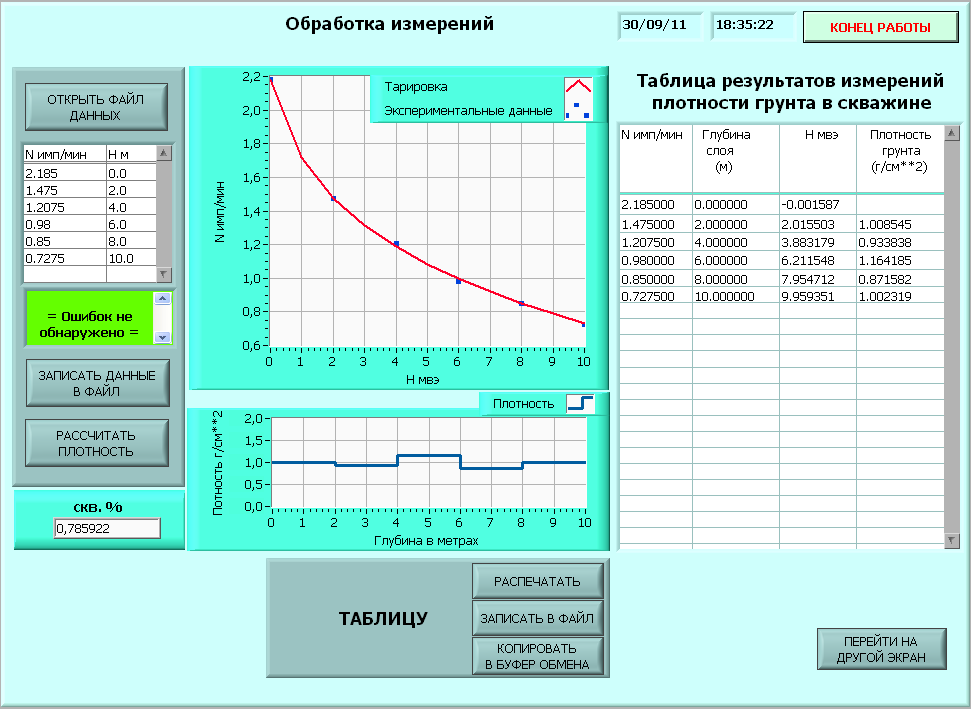
\includegraphics [scale=0.35] {operator_results}
  \caption{Интерфейс оператора по обработке измеренных данных} 
  \label{img:operator_results} 

\end{figure}


При анализе структуры созданного ПО выявлена возможность более тесной интеграции с пультом управления. Это позволило бы автоматизировать ввод данных, их оперативный обсчет и управление временем измерений.

\subsection{Метод определения неоднородностей в почве}
\clearpage